\documentclass{article}
\usepackage[a4paper,margin=1in]{geometry}

\title{Fast and accurate protein false discovery rates on human
proteome study scale with Percolator 3.0}

\author{Matthew The,\\
Science for Life Laboratory,\\
School of Biotechnology,\\
Royal Institute of Technology - KTH,\\
Box 1031, 17121 Solna,\\ Sweden
\and 
Michael J. MacCoss,\\
Department of Genome Sciences,\\
School of Medicine,\\
University of Washington,\\
Seattle, Washington 98195,\\ United States of America
\and 
William S. Noble,\\
Department of Genome Sciences,\\
School of Medicine,\\
University of Washington,\\
Seattle, Washington 98195,\\ United States of America
\and
Lukas K\"{a}ll\\
Science for Life Laboratory,\\ School of Biotechnology,\\
Royal Institute of Technology - KTH\\ 
Box 1031, 17121 Solna,\\ Sweden}

\usepackage{setspace}
\usepackage{amsmath}
\usepackage{url}
%\usepackage{bbm}
\usepackage{dsfont} % preferrred over bbm in submission system
\usepackage{graphicx}
\usepackage[outdir=./img/]{epstopdf}
\usepackage{epsfig}

\begin{document}

\maketitle

\doublespacing

Keywords: mass spectrometry - LC-MS/MS, statistical analysis, 
data processing and analysis, protein inference, simulation


\newpage

\begin{abstract} 
Percolator is a popular tool to assign reliable statistics, such as
q-values and posterior error probabilities, to peptides and peptide
spectrum matches (PSMs) using search results from mass
spectrometry-based proteomics experiments. Percolator's processing
speed has been sufficient for typical data sets with hundreds of
thousands of PSMs. With our new scalable approach, we can now also
analyze millions of PSMs in a matter of minutes on a commodity
computer. Furthermore, with the increasing awareness for the need for
reliable statistics on the protein level, we compared several
easy-to-understand protein inference methods and implemented the best
method in the Percolator package. We used Percolator 3.0 to analyze
the data from a recent study of the draft human proteome containing 20
million spectra (PM:24870542).
\end{abstract}

\newpage

\section*{Introduction}

Percolator~\cite{kall2007} has played a prominent part in the analysis
pipelines of shotgun proteomics experiments for the last decade, by
post-processing the results from database search engines such as
SEQUEST~\cite{eng1994}, MASCOT~\cite{cottrell1999},
X!Tandem~\cite{craig2004tandem} and MS-GF+~\cite{kim2008}. Not only
does Percolator often give a significant boost in the number of
significant peptide spectrum matches (PSMs) or peptides, it also
provides a consistent statistical framework in which to interpret the
search results. As Percolator's running time is usually much lower
than that of the search engine, applying it as a post-processing step
should be a no-brainer. As part of the continuous development and
support of the Percolator package, we present two major additions
aimed at supporting analysis of studies on the scale of the human
proteome~\cite{kim2014draft, wilhelm2014mass}.

As advances in technology are causing shotgun proteomic experiments to
become progressively easy and affordable to carry out, the amount of
data per study will keep rising steadily. While previous versions of
Percolator are able to process the data from the vast majority of
current studies in a decent time frame, certain limitations have come
into sight for laboratories without access to an above average
commodity computer. When processing millions of PSMs, the majority of
Percolator’s processing time is spent on training support vector
machines (SVMs). One could, however, surmise that the performance of
the SVM would plateau pretty fast as a function of the number of input
PSMs. Here, we propose to use Percolator’s semi-supervised learning
algorithm to train SVMs on only a random subset of the PSMs and used
the resulting score vectors to evaluate the rest of the PSMs.

Second, protein-level accuracy estimates have been on our feature wish
list for quite some time now. One of the major obstacles was the
question of how to deal with shared peptides and protein grouping. An
implementation of Fido~\cite{serang2010efficient} has been part of the
Percolator package for quite some time now and addressed these two
issues, but is too computationally intensive on large-scale
datasets with many shared peptides. On the other hand, large-scale
studies have a deep coverage of the present peptides and therefore
identify many peptides that uniquely identify a protein. This
provides the option of ignoring shared peptides altogether and makes
the task of protein inference much simpler and intuitive. Here, we
compared several easy-to-understand protein inference strategies that
only use these peptides that uniquely identify a protein and
implemented the best candidate in the Percolator package.

\section*{Methods}

We downloaded a set of spectra, comprising $2212$ runs on $17$ adult
tissues, $7$ fetal tissues, and $6$ hematopoietic cell types with a
total of $21$ million spectra from~\cite{kim2014draft}. The
investigated peptides were analyzed on an LTQ Orbitrap Velos and Elite
(Thermo Scientific) equipped with an Easy-nLC II nanoflow LC System
(Waters). We will refer to this set as the {\em pandey} set.

Converting the RAW files to MS1 and MS2 files was done with
Proteowizard~\cite{kessner2008}. Next, we assigned high-resolution
precursor masses and charges using information from the precursor
scans with Hardkl\"{o}r \cite{hoopmann2007} followed by Bullseye
\cite{hsieh2009}, through the Crux 2.0 package
interface~\cite{mcilwain2014}. This was followed by a database search
against the human Swissprot and Swissprot+Ensembl databases
(accessed: 2015 Nov 12) using the Tide search engine, again through
the Crux interface. The same search parameters as
in~\cite{kim2014draft} were used, with the exception of not
using cyclization of N-terminal glutamine as a variable modification,
using semi-tryptic searches and using Tide's default fragment
tolerance. For the decoy proteins, we reversed the target
protein sequences. Separate searches were done on the target and decoy
protein database, resulting in a total of $73$ million target and
decoy PSMs.

For assessment of the accuracy of protein-level FDR estimates we also
downloaded two sets of spectra from Human Du145 prostate cancer cells
and Yeast, collected on an LTQ Orbitrap Velos (Thermo Scientific), as
described in Moruz {\em et  al.}~\cite{moruz2013}.  We will refer to
these sets as the {\em hm\_human} and {\em hm\_yeast} sets.
%FIXME: this is copied ad verbatim from the MaRaCluster paper

The normal Percolator's semi-supervised learning algorithm randomly
splits the training set in $3$ folds and computes $3$ scoring vectors,
each trained on $2$ of the $3$ folds and tested on the remaining
fold. The final scores are then calculated using the scoring vector
where the PSM was in the test set. To implement subset scoring, we
simply applied the normal training algorithm on a random subset of the
PSMs, resulting in $3$ scoring vectors. However, instead
of scoring using only a single scoring vector, we now calculate each
PSM's score as the average of the scores from the $3$ scoring vectors.

To characterize the behavior of the scoring vectors based on subsets
of the PSMs, we evaluated the performance for different sizes of the
random subset. Preliminary results showed that including target and
decoy PSMs belonging to the same spectrum together during the
selection of random subsets gave a more stable performance than
sampling without taking this into account. Therefore this strategy was
applied in the random sampling process. For each random subset
size, we calculated the mean and standard deviation over $10$
randomized runs of the number of PSMs and peptides with $q$ value
below $0.001$.

Before applying the protein inference methods, we used the approach to
handling shared peptides from {\em Nesvizhskii et
al.}~\cite{nesvizhskii2003statistical}. Here, proteins are grouped
that are indistinguishable based on their theoretical proteolytically
digested peptides, rather than their experimentally discovered
peptides. We retain the peptides that are unique to such a protein
group, rather than to a single protein. Especially for databases
containing many proteoforms for a gene, this can decrease the number
of shared peptides considerably.

%FIXME: add citation for multiplication of PEPs
We compared several straightforward protein inference methods:
Fisher’s method for p-value combination, the picked target-decoy
strategy~\cite{savitski2015scalable}, and the product of peptide-level
posterior error probabilities (PEPs). We assessed the performance of
the methods on the {\em pandey} set, as well as on the {\em hm_yeast}
and {\em hm_human} sets. We assessed the accuracy and stability of FDR
estimates on the {\em hm\_yeast} data set by using a {\em sample} and
{\em entrapment} database~\cite{granholm2013determining}. The draft
human proteome data could give us an indication of the performance on
real data. We calculated false discovery rate (FDR) estimates from
p-values for Fisher’s method, and using target-decoy models for all
other methods.

\section*{Results}

Searching all $73$ million target+decoy PSMs resulted in $7\,928\,551$
significant PSMs and $298\,095$ unique target peptides at a $q$ value
threshold of $0.01$. Using subsets of even just $100\,000$ PSMs
($0.14\%$) for SVM training did not reduce the number of identified
peptides and generally even slightly increased this number. The
standard deviation of the randomized runs for a fixed subset size did
increase when taking increasingly smaller subsets, but this effect was
limited. By using a subset of $500\,000$ PSMs to train the SVM,
Percolator’s runtime was reduced from several hours to under $10$
minutes.

\begin{figure}[!htp]
\begin{center}
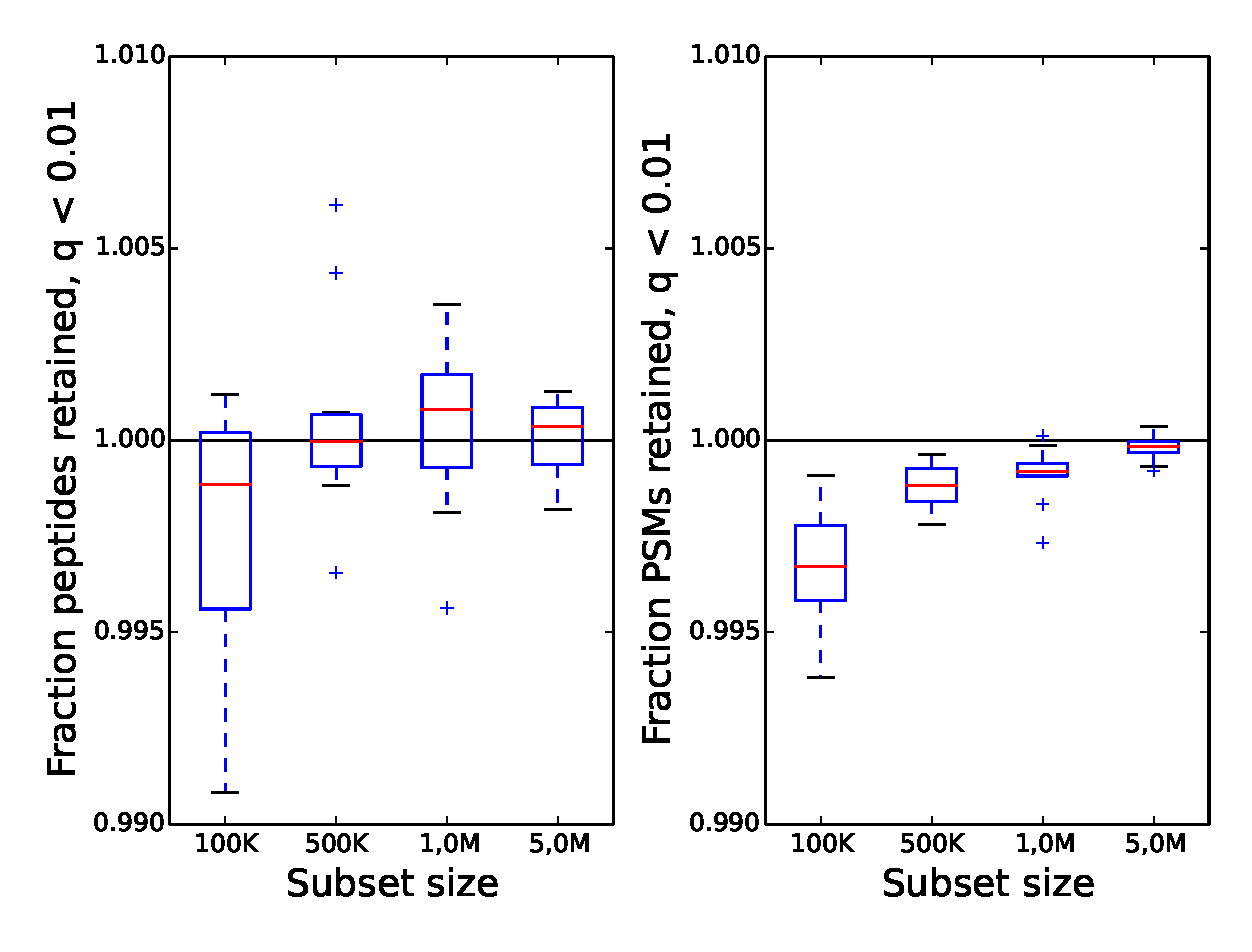
\includegraphics[width=0.6\linewidth]{./img/subset-performance}
\caption{\label{fig:subset}\textbf{Using subsets of the $73$ million
target+decoy PSMs for SVM training retains the number of significant
PSMs and peptides as training using the full set.} We used
$10$ random subsets each of $100\,000, 500\,000, 1\,000\,000$ and
$5\,000\,000$ PSMs to train the SVMs and scored all $73$ million PSMs
using the resulting support vectors. We plotted the ratio of
significant PSMs and peptides at a $q$ value threshold of $0.01$ as
the fraction compared to using the full training set of $73$ million
PSMs. The number of significant PSMs and unique peptides does not drop
significantly for even subsets of $100\,000$ PSMs.}
\end{center}
\end{figure}


% FIXME: table with duplicate/fragment protein statistics

While Fisher’s method gave the most robust FDR estimates, it
identified $5-10\%$ fewer proteins than the picked target-decoy
strategy and product of PEPs. These two strategies did give reasonably
accurate FDR estimates but were more sensitive to errors in the
peptide identification. 

% FIXME: accuracy plot for protein inference methods

For the draft human proteome set, at $1\%$ FDR, the picked
target-decoy strategy identified $12\,300$ proteins, multiplication of
PEPs $11\,600$ and Fisher’s method only $8\,800$. From these results
we concluded that the picked target-decoy strategy was the superior
alternative and implemented this in the newest Percolator package.

% FIXME: table with Pandey number identified proteins

\section*{Discussion}


\section*{Acknowledgements}

%FIXME: add acknowledgement to Uppmax?

\bibliography{percolator}{} 
\bibliographystyle{plain}

\end{document}
